\chapter[Force and scenario centric]{Avoidance with criterion max $F_{c,y}$ as an exercise with both a scenario-centric and a force-centric perspective}

To determine the avoidance with criterion max $F_{c,y}$ (force (control force) centric) and $F_{Y}$ (vehicle centric),  OCPs with the following cost functions are formulated:
\begin{align}
    \text{Min}\ t & \quad\text{topt}\\
    \text{Max}\ \int_{t_s}^{t_f} F_{c,y}(t) dt & \quad\text{Fcopt}\\
    \text{Max}\ \int_{t_s}^{t_f} F_{Y}(t) dt & \quad\text{Fyopt}
        % \text{Min}\ t & \text{topt}\\
        % \text{Max}\ \int_{t_s}^{t_f} F_{c(y)} dt & \text{Fcopt}\\
        % \text{Max}\ \int_{t_s}^{t_f} F_{Y} dt & \text{Fyopt}
\end{align}

A double track (DT) model is used with $F_{x(i)}$ as the control inputs, where $i = 1,\ 2,\ 3,\ 4$, and 
\begin{align}
    \begin{array}{cl}
        F_{x(1)} = F_{x(2)} = F_{x(f)}, & -F_{f(\text{max})} \leq F_{x(f)} \leq F_{f(\text{max})}, \\
        F_{x(3)} = F_{x(4)} = F_{x(r)}, & -F_{r(\text{max})} \leq F_{x(f)} \leq 0,
    \end{array}
\end{align}
where $F_{f(\text{max})}$ and $F_{r(\text{max})}$ are detemined using 
\begin{align}
    F_{f(\text{max})} &= \mu_{x(f)}F_{z(f)}, & F_{r(\text{max})} &= \mu_{x(r)}F_{z(r)},
\end{align}
and $F_{z(f)}$, $F_{z(r)}$ are determined using \eqref{eq:prob2_maxforce_DT}.

The obstacle is given by the following relation, 
\begin{align}
    \left(\frac{x - X_a}{R_1}\right)^n + \left(\frac{y}{R_2}\right)^n \geq 1,
\end{align}
A dimensionless parameter $\gamma$ is calculated using 
\begin{align}
    \gamma &= \arctan\left(\frac{B}{A}\right), & B &= R_2, & A&= X_a - R_1.
\end{align}
This is rather conservative and aids the vehicle to avoid the obstacle. 
$\gamma$, in this case, is 9.5$^\circ$ ($\geq 16.7^\circ$), and considering wet asphalt (see \ref{sec:prob3_STrbrk}), then evading is a better option. 
It is worth mentioning that $\gamma$ is calculated using the obstacle height rather than the lateral distance where the vehicle and the obstacle intersect. 
This is to provide a better chance for the vehicle to avoid the obstacle. 

The angle of the obstacle ($\theta_v$) is the angle between the component of the global force ($F_{x}$) and the velocity vector and is calculated using 
\begin{align}
    \theta_v = \frac{\gamma + \arcsin\left(3\sin\left(\gamma\right)\right)}{2}.
\end{align}
The control force vectors ($F_{c,x}$ and $F_{c,y}$) are calculated using
\begin{align}
    \begin{bmatrix}
        F_{c,x}(t) \\
        F_{c,y}(t)
    \end{bmatrix} &=
    \begin{bmatrix}
        \cos\left(\theta_v\right) & \sin\left(\theta_v\right) \\
        -\sin\left(\theta_v\right) & \cos\left(\theta_v\right)
    \end{bmatrix}
    \begin{bmatrix}
        \cos\left(\psi(t)\right) & -\sin\left(\psi(t)\right) \\
        \sin\left(\psi(t)\right) & \cos\left(\psi(t)\right)
    \end{bmatrix}
    \begin{bmatrix}
        F_{X}(t)\\
        F_{Y}(t)
    \end{bmatrix}.
\end{align}

A solution to the optimization problem is determined using the homotopic approach. The OCP is solved for the topt case and this solution is used as initial guesses for Fcopt and Fyopt. 

The constraints to the optimization problem are 
\begin{align}
    \begin{array}{ccccc}
        |\delta| \leq \delta_\text{max} & |\dot\delta| \leq \dot\delta_\text{max} & 
        0 \leq t \leq t_{\text{max}} & 0 \leq y \leq y_\text{max} & 0 \leq x \leq x_\text{max}
    \end{array}
\end{align}

\begin{table}[h!]
    \centering
    \begin{subtable}{0.3\textwidth}
        \begin{tabular}{c|c}
            Parameter & Value\\
            \hline
            $X_a$ & 20\,m\\
            $R_1$ & 2\,m\\
            $R_2$ & 3\,m\\
            $n$ & 12
        \end{tabular}
        \caption{Obstacle parameters}
        \label{tab:obst_pprty}
    \end{subtable}
    \begin{subtable}{0.3\textwidth}
        \begin{tabular}{c|c}
            Parameter & Value\\
            \hline
            $m$ & 2100\,kg\\
            $l_f$ & 1.3\,m\\
            $l_r$ & 1.5\,m\\
            $w$ & 0.8\,m\\
            $g$ & 9.81\,m/s\textsuperscript{2}\\
            $I_{zz}$ & 3900\,kg\textsuperscript{2}
        \end{tabular}
        \caption{Vehicle parameters}
        \label{tab:veh_pprty}
    \end{subtable}
    \begin{subtable}{0.3\textwidth}
        \begin{tabular}{c|c}
            Parameter & Value\\
            \hline
            $\delta_\text{max}$ & 30$^\circ$\\
            $\dot\delta_\text{max}$ & 45$^\circ$/s\\
            $v_x(t_0)$ & 20\,m/s\\
            $t_{\text{max}}$ & 2\,s\\
            $y_{\text{max}}$ & 7.5\,m\\
            $y_{\text{max}}$ & 20\,m\\
            $y(t_f)$ & 3\,m
        \end{tabular}
        \caption{Optimization constraints}
        \label{tab:const_pprty}
    \end{subtable}
    \caption{Obstacle-, vehicle-parameters and optimization constrains.}
\end{table}

The optimal trajectories for the three OCPs are shown in Figure~\ref{fig:prob6_traj}. From the figure, it is clear that the trajectories for the three cases are similar. An expected solution should be that the Fcopt and Fyopt solution avoids the obstacle with some room to spare. It is difficult to say why this is happening. However, a clue is when comparing the solution of Fcyopt and OCP solution with the cost function to maximize the input velocity (vopt). In this case, the vopt and Fcopt should have identical trajectories and this is shown in Figure~\ref{fig:prob6_v2_traj}. 
\begin{figure}[h!]
    \centering
    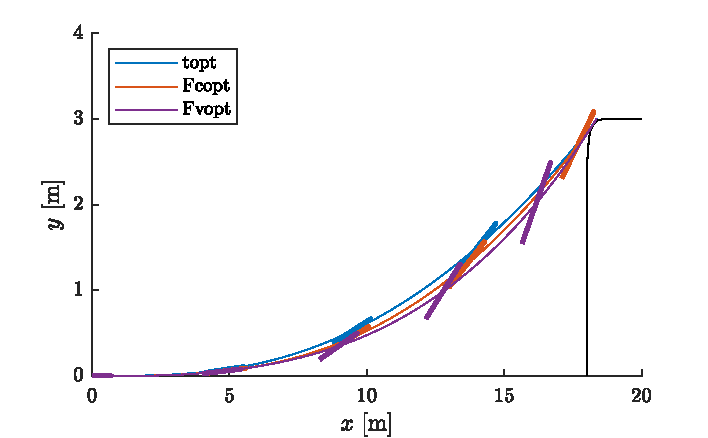
\includegraphics{figures/prob6_traj.pdf}
    \caption{Trajectories for time (topt), control force centric (Fcopt), and vehicle centric (Fyopt) optimal obstacle avoidance maneuver. The rectangles indicate the position and orientation of the vehicle every 0.25\,s.}
    \label{fig:prob6_traj}
\end{figure}
\begin{figure}[t!]
    \centering
    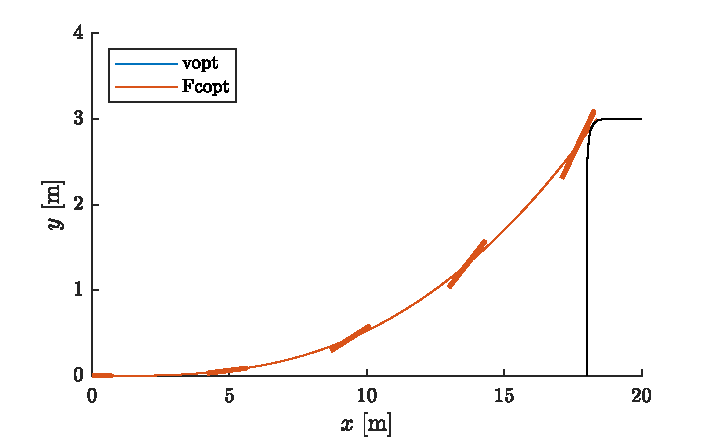
\includegraphics{figures/prob6_v2_traj.pdf}
    \caption{Trajectories for input velocity (vopt) and control force centric (Fcopt) optimal obstacle avoidance maneuver. The rectangles indicate the position and orientation of the vehicle every 0.25\,s.}
    \label{fig:prob6_v2_traj}
\end{figure}
\clearpage
The forces are shown in Figure~\ref{fig:prob6_forces}. From the figure, $F_{c,y}$ is maximized at every time instant for the Fcopt case. At $x = 5$\,m, $F_{c,y}$ for topt is greater than Fcopt because $|F_{c,x}|$ for topt is lower than for Fcopt. Figure~\ref{fig:prob6_detailed} shows the vehicle model variables for all the there OCPs. From the figure, it can be seen that the velocity for the topt stays constant. In the Fopt case, the velocity reduces significantly until 15\,m (as the vehicle approaches the object and $\varphi_v(t) \rightarrow \theta_v$), and then the rate of change of velocity reduces. The lateral slips for the Fyopt case are the highest because Fy is maximized at every time instant. The lateral forces on the wheels for Fcopt and Fyopt are similar until 15\,m and as the vehicle approaches the obstacle ($\varphi_v(t) \rightarrow \theta_v$), in Fcopt, $F_Y$ starts to reduce and $F_X$ starts to increase. However, Fyopt tries to make the vehicle go around in circles. 

\begin{figure}[h]
    \centering
    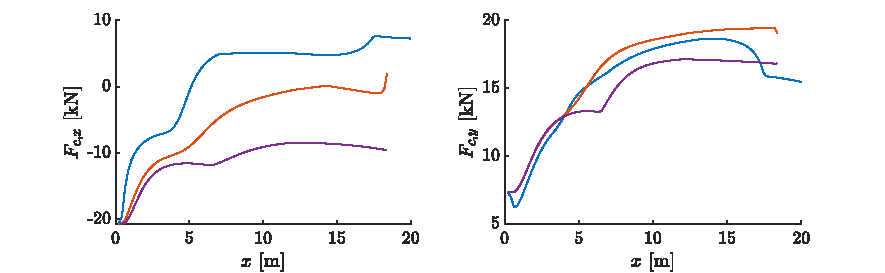
\includegraphics{figures/prob6_forces.pdf}
    \caption{Control forces for the time (topt), control force centric (Fcopt), and vehicle centric (Fyopt) optimal obstacle avoidance maneuver.}   
    \label{fig:prob6_forces}
\end{figure}

\begin{figure}[h]
    \centering
    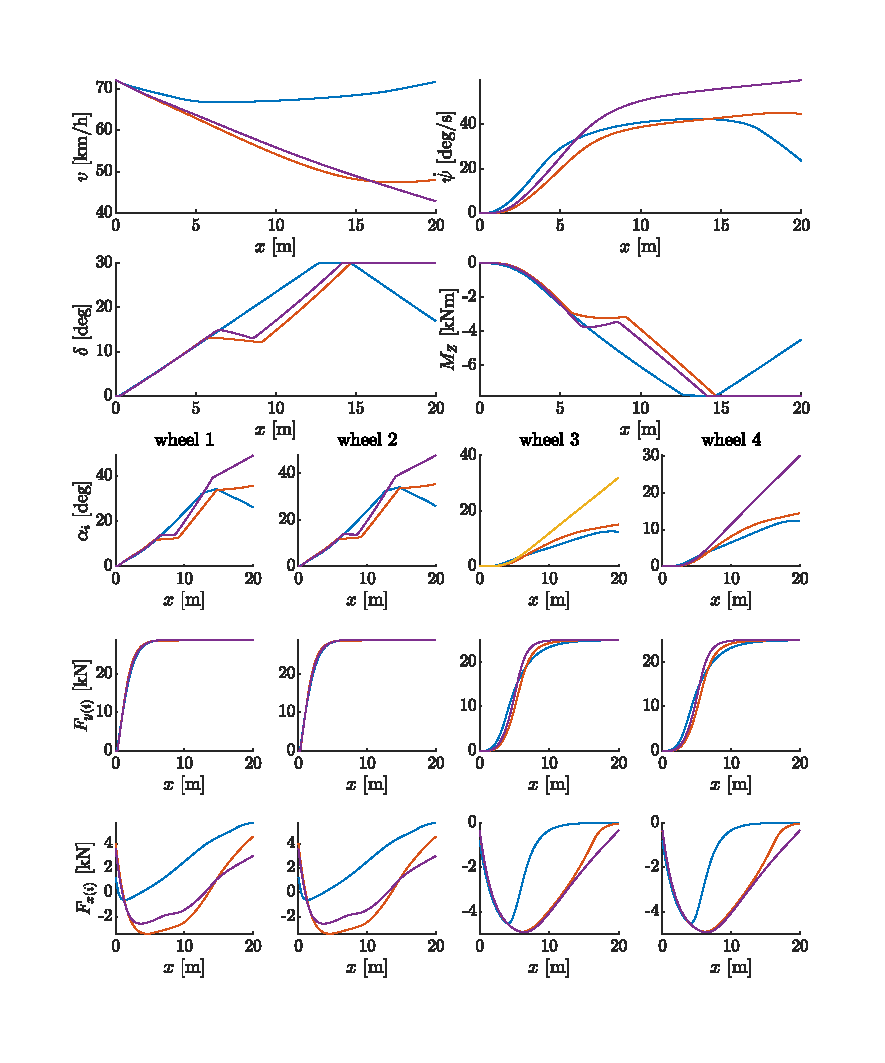
\includegraphics{figures/prob6_detailed.pdf}
    \caption{Variables of the vehicle model during the time (topt), control force centric (Fcopt), and vehicle centric (Fyopt) optimal obstacle avoidance maneuver.}   
    \label{fig:prob6_detailed}
\end{figure}

\noindent\fbox{%
    \parbox{\textwidth}{%
        \textbf{Some reflections}: \newline
        While analyzing the results, for some reason, $F_Y$ is negative, and $F_X$ seems to be similar for all three cases and the reason for this is unknown. Probably this is some bug in the model that can be fixed for future versions. \newline
        I was expecting the trajectories for the Fcopt and Fyopt solutions to avoid the obstacle with a significant distance to the vehicle. When the optimization was rerun with a free value for the initial velocity, then this is observed. However, the initial velocities for the three OCPs are different, especially for Fvopt. The solver struggles to converge to a solution and often throws a restoration failed error message. A homotopic approach can be used to guide ipopt in the desired direction. 
    }
}



% \section{The particle model}
% The angle of the obstacle ($\psi_v$) is the angle between the component of the global force ($F_{x}$) and the velocity vector and is calculated using 
% \begin{align}
%     \psi_v(t) &= \frac{dy(t)}{dx(t)}.
% \end{align}
% The vehicle centric control force vectors ($F_{c,x}$ and $F_{c,y}$) are calculated using
% \begin{align}
%     \begin{bmatrix}
%         F_{v,x}(t) \\
%         F_{v,y}(t)
%     \end{bmatrix} &=
%     \begin{bmatrix}
%         \cos\left(\psi_v(t)\right) & \sin\left(\psi_v(t)\right) \\
%         -\sin\left(\psi_v(t)\right) & \cos\left(\psi_v(t)\right)
%     \end{bmatrix}
%     \begin{bmatrix}
%         F_{x}(t)\\
%         F_{y}(t)
%     \end{bmatrix}.
% \end{align}
% $\psi_v$ when the vehicle just touches the obstacle at time $t_o$ is calculated using 
% \begin{align}
%     \theta &= \psi_v(t_o)\vert_{f_o(x,y)=1}.
% \end{align}
% The scenario centric control force vectors ($F_{c,x}$ and $F_{c,y}$) are calculated using
% \begin{align}
%     \begin{bmatrix}
%         F_{c,x}(t) \\
%         F_{c,y}(t)
%     \end{bmatrix} &=
%     \begin{bmatrix}
%         \cos\left(\theta\right) & \sin\left(\theta\right) \\
%         -\sin\left(\theta\right) & \cos\left(\theta\right)
%     \end{bmatrix}
%     \begin{bmatrix}
%         F_{x}(t)\\
%         F_{y}(t)
%     \end{bmatrix}.
% \end{align}

% The optimization results for the force and scenario centric are presented in Figure~\ref{fig:prob5_res}. From the figure, it is clear that the control force magnitude for the $y$ direction is constant for both the scenario-, vehicle-, and global-centric. However, the $x$ is different for scenarios, which is rather intuitive.

% \vspace{5pt}
% \noindent\fbox{%
%     \parbox{\textwidth}{%
%         \textbf{Some reflections}: \newline
%         It is worth mentioning that, in Figures~\ref{fig:num_sol_opt_avoid_PM_res_pic} and ~\ref{fig:prob5_res}, the intersection occurs at $t = 1.07$s. However, the vehicle starts to decelerate in the $y$-direction at around 1\,s, when $x = 20$\,m. This is probably due to the order of sharpness of the obstacle. when the degree of the super ellipse (obstacle model) is reduced, the vehicle starts to decelerate earlier and smoother. 
%     }%
% }

% \begin{figure}[h!]
%     \centering
%     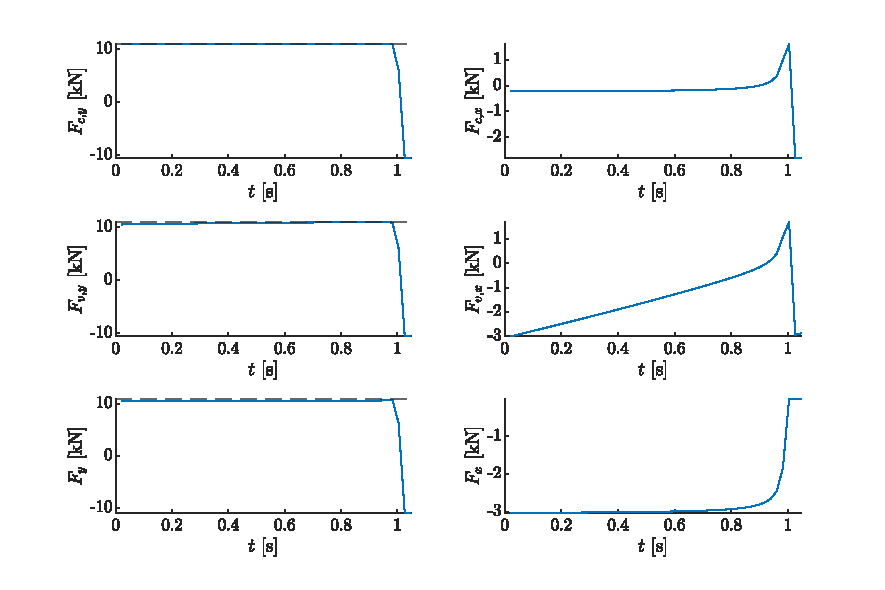
\includegraphics{figures/prob5_opt_avoid_controlforce.pdf}
%     \caption{Criteria for max $F_{c,y}$ for both a scenario-centric and a force-centric perspective.}
%     \label{fig:prob5_res}
% \end{figure}

\subsection{Code}
The source codes for this problem can be found at \newline \href{https://github.com/arvba41/optimal_vehicle_maneuvers/blob/main/uppgift/ugf5/force_centric_and_scenario_centric_PM.m}{https://github.com/arvba41/optimal\_vehicle\_maneuvers}.